\documentclass[11pt,border=5pt]{standalone}
\usepackage{fontspec}
\setmainfont{cmunrm.otf}[BoldFont=cmunbx.otf,ItalicFont=cmunti.otf,BoldItalicFont=cmunbi.otf]
\usepackage{amsmath}
\usepackage{unicode-math}
\setmathfont{NewCMMath-Regular.otf}
\usepackage{tikz}
\usetikzlibrary{arrows.meta,patterns,angles,quotes}
\begin{document}
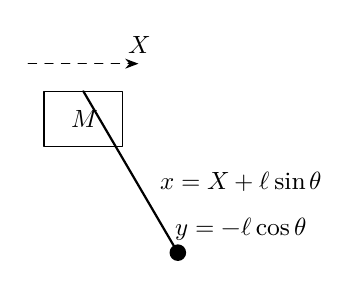
\begin{tikzpicture}[>=Stealth,font=\small,line cap=round,line join=round]
\draw[fill=white] (-0.5,-0.35) rectangle (0.5,0.35);
\node at (0,0) {$M$};
\draw[thick] (0,0.35) -- (1.2,-1.7);
\fill(1.2,-1.7) circle(3pt);\draw[->,thin,dashed] (-0.7,0.7) -- (0.7,0.7) node[above] {$X$};
\node at (2,-0.8) {$x=X+\ell\sin\theta$};
\node at (2,-1.4) {$y=-\ell\cos\theta$};

\end{tikzpicture}
\end{document}
